\chapter{Program descriptions}
This chapter contain the description of the various input parameters, file formats, and output files for the NISE code.
\section{Units}
The code use wavenumbers (cm$^{-1}$) for frequencies and times are in femtoseconds (fs). Users are discouraged from trying to use other units at this may lead to numerical instabilities or unit conversion errors. The transition
dipoles and transition polarizabilities may be given in any desired units. The final results will scale accordingly. However, for using the on-the-fly coupling calculations the transition dipoles should be provided in Debye and positions should be provided in \AA ngstr\"{o}m. 

\section{Programs}
Overview over programs for calculating spectra and analysis:\\
\begin{description}
\item [translate] [Convert Hamiltonian and dipole trajectory between different formats.]
\item [NISE] [General code for calculating spectra]
\item [2DFFT] [Do the 2D Fourier transform]
\end{description}

\section{Translate}
The Hamiltonian \textbf{must} be saved in binary format (GROBIN/SKIBIN) for use in the NISE program.
The translate program convert between different formats. The program also allows selecting specific sites in a Hamiltonian file and modification of the fundamental frequencies corresponding to isotope labeling. The input file format is:
\begin{description}
\item[InputEnergy] [filename]
\item[InputDipole] [filename (only needed for GRO/SKI formats)]
\item[InputDipoleX] [filename (only needed for MIT format)]
\item[InputDipoleY] [filename (only needed for MIT format)]
\item[InputDipoleZ] [filename (only needed for MIT format)]
\item[InputAnharm][filename (only needed for SKI format)]
\item[InputOverto][filename (only needed for SKI format)]
\item[InputAlpha][filename (only available for GRO format)]
\item[OutputEnergy] [filename]
\item[OutputDipole] [filename (only needed for GRO/SKI formats)]
\item[OutputDipoleX] [filename (only needed for MIT format)]
\item[OutputDipoleY] [filename (only needed for MIT format)]
\item[OutputDipoleZ] [filename (only needed for MIT format)]
\item[OutputAnharm][filename (only needed for SKI format)]
\item[OutputOverto][filename (only needed for SKI format)]
\item[OutputAlpha][filename (only available for GRO format)]
\item[Singles] [number of oscillators]
\item[Doubles] [number of doubly excited states]
\item[Skip][Doubles=Neglect doubly excited states, needed for SKIBIN]
\item[Length] [number of timesteps in the trajectory files]
\item[Anharmonicity][A fixed anharmonicity. Only needed for generating GROBIN file from format without double excited states.]
\item[InputFormat] [GROBIN/GROASC/MITASC/SKIBIN]
\item[OutputFormat] [GROBIN/GROASC/MITASC/SKIBIN]
\item[Modify][Leave this out if you do not wish to modify the Hamiltonian. This keyword requires that the keywords Select, Label, and Shift are also given.]
\item[Select] [Number of amide units to include, if selected number is less than the number of units in the original a list of the units to include should be given on the following line (i.e. 0 1 2 3 5 if 6 units are in the original and we want unit 4 excluded) Note that Singles should be the number of residues in the original file. This keyword is only used if the Modify keyword is used.]
\item[Label] [On the following line the for each selected unit the isotope labeling is given (0=native, 1=C13, 2=O18) C13 gives a 41 wavenumber frequency shift and O18 gives a 60 wavenumber shift in this implementation. This keyword is only used if the Modify keyword is used.]
\item[Shift] [On the following line for each selected unit a frequency shift can be provided. This can be used for modifying proline or terminal frequencies or for isotope labeling. This keyword is only used if the Modify keyword is used.]   
\end{description}

\subsection{File formats}
GROBIN is the binary format needed for use with the NISE program. This contains information on the energy of both singly and doubly excited states and allows for fluctuating anharmonicities.
GROASC is a text readable format.
MITASC and MITTXT are text formats used by the MIT static spectrum code.
SKIBIN is a binary format used by the Skinner group. It contain the singly excited states and a
separate file for fluctuating anharmonicities and a file for fluctuating overtone transition dipoles.
SPECTRON is a text format used by the Mukamel group SPECTRON code.
The GROBIN format is the only format that allows storing the doubly excited states Hamiltonian. This will be generated automatically using harmonic rules and the anharmonicity given by the Anharmonicity keyword.

\noindent
\underline{GROBIN and SKIBIN:}\\
The GROBIN and SKIBIN formats are very similar.
The energy file has the following format.
For each snapshot in the trajectory they contain first an integer typically containing the number of the snapshot. This integer is not used in the calculation, but can be used for control purposes.
Then the single excited Hamiltonian is given in floats as a tridiagonal upper matrix. For the GROBIN
format the double excited Hamiltonian might be provided afterwards again in a tridiagonal upper matrix.

The dipole file has the following format.
For each snapshot in the trajectory they contain first an integer typically containing the number of the snapshot. This integer is not used in the calculation, but can be used for control purposes.
Then the x components of the transition dipole matrix are given in floats, followed by the y and z components. For the GROBIN format the transition dipole matrix for the single to double transitions may then be given, again with the x components given first. In Figure \ref{fig:filestructure} the format of the file is also illustrated.
\begin{figure}[h!]
\begin{center}
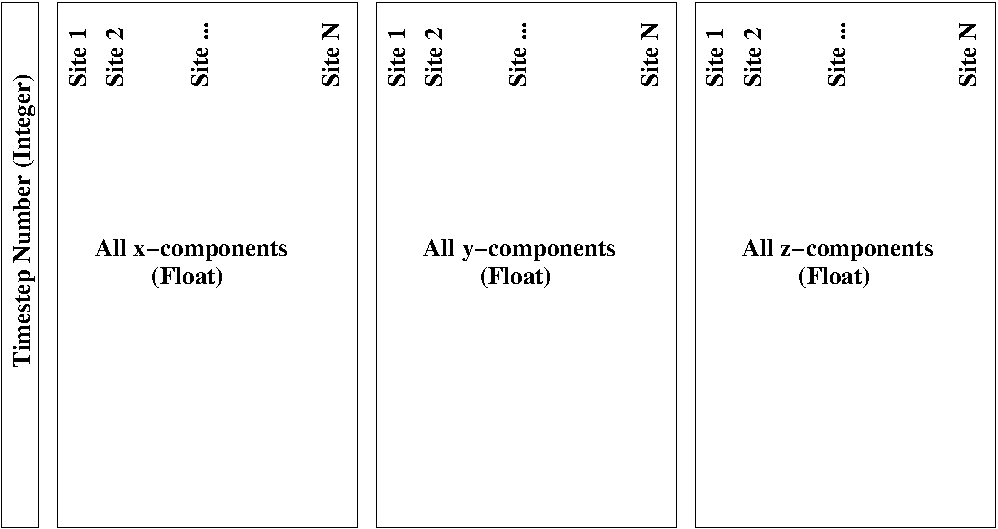
\includegraphics[width=10cm]{file_structure.pdf}
\end{center}
\caption{\label{fig:filestructure}The file structure for the dipole, and position files.}
\end{figure}

The anharmonicity file is only given in the SKIBIN format.
For each snapshot in the trajectory they contain first an integer typically containing the number of the snapshot. This integer is not used in the calculation, but can be used for control purposes.
Then the diagonal anharmonicities are then given in floats.

The overtone file is only given in the SKIBIN format.
For each snapshot in the trajectory they contain first an integer typically containing the number of the snapshot. This integer is not used in the calculation, but can be used for control purposes.
Then the overtone transition dipoles are then given in floats. Only the same site overtone transition dipoles are given. Transitions like $\langle 1\mid\mu\mid 12\rangle$ are determined by the harmonic rules.

The transition polarizability file which is not available in the SKIBIN format 
has the following format. For each snapshot in the trajectory they contain first an integer 
typically containing the number of the snapshot. This integer is not used in the calculation, 
but can be used for control purposes. Then the xx components of the transition polarizability
matrix are given in floats, followed by the yy and zz components. 

The position files are available in the GROBIN format and used to store either the center positions of the chromophores or the positions of the two sites in each chromophore defining the extended dipole coupling. This file is used when calculating CD spectra, excition diffusion, or when using the on-the-fly coupling calculations. The structure of the file is as for the dipole files (see Figure \ref{fig:filestructure}).

\noindent
\underline{GROASC:}\\
The energy file contain one Hamiltonian snapshot for each line. The upper tridiagonal matrix is saved and each number is separated by a space. The transition dipoles are stored in one file. Each line contains one snapshot with the numbers separated by a space. All the x components for one snapshot are stored first followed by the y and z components. Only the single excitation Hamiltonian and the transition dipoles from the ground state to the singly excited state are saved.

\noindent
\underline{MITASC:}\\
The energy file contain one Hamiltonian snapshot for each line. The whole square matrix is saved and each number is separated by a tab. The transition dipoles are stored in one file for each cartesian component. Each line contains one snapshot with the numbers separated by a tab. Only the single excitation Hamiltonian and the transition dipoles from the ground state to the singly excited state are saved.

\noindent
\underline{MITTXT:}\\
The energy file contain one row of the Hamiltonian snapshot for each line. The whole square matrix is saved and each number is separated by a space. Snapshots are separated by an empty line. The transition dipoles are stored in one file for each cartesian component. Each line contains the cartesian coordinates of one transition dipole. The numbers separated by a space. Snapshots are separated by an empty line. Only the single excitation Hamiltonian and the transition dipoles from the ground state to the singly excited state are saved.

\noindent
\underline{SPECTRON:}\\
In the energy file each snapshot is stored after a line containing the word SNAPSHOT and the number
of the snapshot (starting from 1). After this the upper tridiagonal matrix of the Hamiltonian snapshot is stored with one row on each line. The numbers are separated by a space. The dipole file also contain a line with the word SNAPSHOT and the number of that snapshot. This is followed by the transition dipoles stored with the x, y and z components for each site on one line separated by a space. Only the single excitation Hamiltonian and the transition dipoles from the ground state to the singly excited state are saved.


\subsection{NISE (Full nonadiabatic simulation)}
The nonadiabatic linear and third-order response can be simulated with the 'NISE' program utilizing the numerical integration of the Schr\"odinger equation (NISE) approach\cite{Jansen.2006.JPCB.110.22910,Jansen.2009.ACR.42.1405}. The sparse and double excited state propagation is described in \cite{Jansen.2010.JCP.132.224503}.
The coupling propagation scheme is described in \cite{Liang.2012.JCTC.8.1706}.
The program require the Hamiltonian trajectory in binary format.
The NISE program use the following input:\\
\begin{description}
\item [Hamiltonianfile] [File name]
\item [Dipolefile] [File name]
\item [Alphafile] [File name] (Only needed for SFG calculations)
\item [Anharmonicfile] [File name]
\item [Overtonedipolefile] [File name]
\item [HamiltonianType] [Full/Coupling/TransitionDipole/ExtendedDipole] (Full is the default)
\item [Couplingfile] [File name]
\item [PDBfile] [File name]
\item [Length] [Number of snapshots in trajectory] 
\item [Samplerate] [Number of snapshots between ensemble averaging]
\item [Lifetime] [The life time in fs included in 2D response functions]
\item [Homogeneous] [Homogeneous lifetime for exponential apodization in fs, only included after FFT]
\item [Inhomogeneous] [Inhomogeneous lifetime for gaussian apodization in fs, only included after FFT]
\item [Timestep] [The length of each timestep in fs]
\item [RunTimes] [t1 max] [t2] [t3 max, all in timesteps]
%\item [MinTimes] [t1 min] [t2 min] [t3 min, all in timesteps, t1 min and t3 min should be 0]
%\item [MaxTimes] [t1 max] [t2 max] [t3 max, all in timesteps, t2 max should equal t2 min+1]
%\item [TimeIncrement] [dt1] [dt2] [dt3, all in timesteps, default 1]
\item [Threshold][The threshold for the sparse matrix approximation, typical value 0.001]
\item [Anharmonicity] [0 = anharmonicities from file used, all other values result in the use of a fixed anharmonicity with that value]
\item [Singles] [Number of singly excited states]
\item [Propagation] [Sparse/Coupling default is Sparse] (Coupling recommended for fast calculations)
\item [Couplingcut] [Value in cm$^{-1}$ below which the couplings are neglected, default 0, only used in the Coupling propagation scheme. From the 16/8-2022 version couplings below the cutoff are neglected when reading in the Hamiltonian or when it is constructed on the fly. NOTE that before this the approximation was NOT applied during t$_2$ for two-dimensional spectroscopic calculations and it was not used for the Analysis of the Hamiltonian.]
\item [Trotter] [The number of trotter steps in the Paarmann approximation for double excited 
states, 5 recommended for the Sparse propagation scheme, for the Coupling propagation scheme this is the general number of trotter steps the recommended value is then 1 ]
\item [MinFrequencies] [minw1] [minw2] [minw3, all in reciprocal cm]
\item [MaxFrequencies] [maxw1] [maxw2] [maxw3, all in reciprocal cm]
%\item [Static] [Minimum frequency] [Maximum frequency] [Bin size for 1D static spectrum]
\item [Technique] [Absorption / DOS / Luminescence / CD / 2DIR / GBIR / SEIR / EAIR / noEAIR / 2DUVvis / GBUVvis / SEUVvis / EAUVvis / noEAUVvis / Pop / Dif / Ani / Analyse, these techniques are explained in Section \ref{chap:techniques}]
\item [FFT] [Number of points on each axis in 2DFFT, if bigger than max times zero padding is used]
%\item [Timevariables] [1/2/3 First time to Fourier transform, should be 1] [1/2/3 Second time to Fourier transform, should be 3]
\item [Format] [Matlab/Dislin/Gnuplot For Matlab format rephasing and non-rephasing spectra are not added] 
\item [BeginPoint] [The number of the first sample calculated in this run]
\item [EndPoint] [The number of the last sample calculated in this run, if this keyword is left out all samples will be included]
\item [Project] (Should be followed by either two new lines specifying the sites to project on directly in the file or one line specifying the filename of a file to read the site numbers from. In the first case the first line should read Sites [Number] identifying how many sites are included in the projection and the second line with a list of integer numbers identifying the sites included counting from zero. In the other case the following line should read Projectfile [Name], where the file named [Name] contain the number of sites on the first line and then a list of the site numbers.)
\item [PrintLevel] [0 / 1 / 2 ] (Default is 0, the higher number the more detailed (timing) info is given.)
\end{description}

The minimum and maximum frequencies are used for two things. First, the average of minw1 and maxw1 are used to shift the frequencies during the simulation. By shifting all transitions by the
average the oscillations of the time-evolution are reduced and the simulations can be performed with
longer distance between the time points. Second, the output is reduced to frequencies within the
min and the max which reduce file size.

The Lifetime is only applied during the coherence times ($t_1$ and $t_3$ ) according 
to the formula in Ref. \citenum{Liang.2012.JCTC.8.1706}. The waiting time dependence can trivially be accounted for by 
multiplying the whole spectrum with $\exp( -t_2 /T_1 )$. For apodization with an exponential or gaussian function the Homogeneous and Inhomogenious keywords are used. These only change the final spectra and not the response functions. The equations used are
\begin{equation}
R'(t)=R(t)\exp\left(-t/2 t_{\textrm{homo}}-t^2/2 t_{\textrm{inhomo}}^2\right)
\end{equation}
for the linear techniques,
\begin{equation}
R'(t_1,t_2,t_3)=R(t_1,t_2,t_3)\exp\left(-(t_1+t+3)/2 t_{\textrm{homo}}-(t_1-t_3)^2/2 t_{\textrm{inhomo}}^2\right)
\end{equation}
for rephasing signals and
\begin{equation}
R'(t_1,t_2,t_3)=R(t_1,t_2,t_3)
\exp\left(-(t_1+t+3)/2 t_{\textrm{homo}}-(t_1+t_3)^2/2 t_{\textrm{inhomo}}^2\right)
\end{equation}
for non-rephasing signals. As default no apodization is performed. The apodizations are inactive when set to zero.  

The HamiltonianType allow the use of different ways to store the Hamiltonian trajectories. The default setting is Full, where the full Hamiltonian is given in the Hamiltonianfile, if Coupling is specified the couplings are assumed to be constant and given in the Couplingfile. The Hamiltonianfile then contain the trajectory of fluctuating diagonal elements. If TransitionDipole is specified the couplings are calculated on the fly using the transition-dipole coupling scheme. The chromophore positions must then be provided in the Positionfile and the transition-dipoles in the Dipolefile. As for the Coupling method the HamiltonianFile then only contains the diagonal elements. The dipoles are then assumed in Debye and Positions in \AA ngstr\"{o}m. If ExtendedDipole is selected the extended-dipole coupling scheme is used to calculate coupling on the fly. The dipole magnitude is then taken from the Dipolefile. The position of the two transition point-charges must be provided in the Positionfile, with the first point corresponding to odd timepoints and the second point corresponding to even timepoints.

The double excitation Hamiltonian is propagated using the Trotter formula scheme\cite{Paarmann.2008.JCP.128.191103,Jansen.2010.JCP.132.224503}.

During the calculation the program will create a log file called NISE.log. For linear techniques this file will be updated every time a new sample has been calculated. The update contains timing information and
therefore allows for the estimation of when the complete calculation finishes. For 2D techniques the timing information will given directly in the output file tracking the progress percentage.

For exciton diffusion calculations an additional input file containing the site positions is needed.
This file should be named Position.bin and have the following format. The first entry should be the
size of the box in float (all sides are assumed equally long). This is followed by the x, y, and z coordinates for each site again in floats. After the coordinates of the first snapshot the coordinates
for the second follows directly and the coordinates for all snapshots should be stored.

%For SFG, 2DSFG, and linear dichroism calculations the principle axis is assumed to be the z-axis. The SFG calculations only support the calculation of $\chi^{(2)}_{zzz}$ and $\chi^{(2)}_{xxz}$, which require the diagonal elements of the transition polarizability tensor (given in the alpha file). For 2DSFG $\chi^{(4)}_{zzzzz}$ and $\chi^{(2)}_{zzzxx}$ are currently calculated.

\subsection{Program output}
The linear absorption calculation provides the linear response function in time domain in the file TD\_Absorption.dat 
and the linear dichroism response function in time domain in the file RLD.dat. The first 
column is the time in femto seconds. The other columns are the real and imaginary parts 
of the response function. It is recommended to check that these have decayed to a small 
value close to zero in the calculated time interval. If this is not the case the system has 
not lost its coherence within the time determined by t1 max and the spectrum will be 
too broad. The linear absorption is given in the file Absorption.dat and the linear dichroism in 
the file LDIR.dat. The first line is the frequency in wavenumbers, the second line is the 
absorption spectrum, and a third line contain zeroes. For the linear dichroism calculation 
the z-axis is assumed to be the unique axis. 

%The SFG calculation provides the second order response function in time domain in  the files RSFG\_zzz.dat and RSFG\_xxz\_yyz.dat. The first column is the time in femto seconds. The other columns are the real and imaginary parts of the response function.  It is recommended to check that these have decayed to a small value close to zero in the calculated time interval. If this is not the case the system has not lost its coherence within the time determined by t1 max and the spectrum will be too broad. The frequency domain response functions are given in the files SFG\_zzz.dat and SFG\_xxz\_yyz.dat. The first line  is the frequency in wavenumbers, the second line is the absorption spectrum, and a third line contain zeroes. The z-axis is assumed to be the unique axis.

The 2D calculations (2DIR and 2DUVvis) provides the files R(par/per/cro)(I/II).dat. These files contain the time domain
third-order response functions for different polarization directions \cite{Hochstrasser.2001.CP.266.273,Zanni.2001.PNAS.98.11265}.
The first three columns are the times t1, t2, and t2 in femtoseconds.
The two last columns are the real and imaginary parts of the response functions. The frequency domain
response functions are found using a double Fourier transform (see section \ref{sec:Fourier}).
It is recommended to check that the response function has decayed within the calculated time intervals.

%The 2DSFG calculation stores the $\chi^{(4)}_{zzzzz}$ signal in Rpar(I/II).dat, while the $\chi^{(4)}_{zzzyy}$ signal is stored in Rper(I/II).dat. The files are essentially identical to the normal 2D response files and are Fourier transformed in the same way (see section \ref{sec:Fourier}).

The population transfer calculation provides two files. Pop.dat contain two columns. The first is the
time in femtoseconds the second is the probability that if a site was initially excited it is still excited
after the given time. This is averaged over all sites. The file PopF.dat contain more detailed information.
The first column is the time. The following columns are the probability that if a particular site was excited
initially other sites are excited later. The first N columns are the populations of the N sites following an initial excitation of the first site. Then follows the populations after excitation of the second site etc. This file might be a very large file for big systems.

For the exciton diffusion the output file is Dif.dat It has three columns. The first is the time in femto seconds. The second column is the mean square displacement of the wave function assuming that
one site is initially excited. The third column is the mean square displacement of the center of the 
wave function assuming that one site is initially excited. The program averages over all sites as
initial sites. One should be aware that periodic boundary conditions are applied in this calculation
and the mean square displacements will saturate \cite{Jansen.2010.JCP.132.224503}.

For the integrated anisotropy calculation the output file is Ani.dat. It has three columns. The first is the time in femtoseconds. The second is the integrated anisotropy and the last is the orientational correlation function.

The Hamiltonian analysis provides the delocalization length/size according to the def- 
inition of Thouless \cite{Thouless.1974.PR.13.93} directly in the program standard output. 

\section{Fourier transform \label{sec:Fourier}}
The 2DFFT program use the same input as the NISE program.
Fourier transformed response is written in files named Rw(par/per/cro).(I/II).dat, where par, per, and cro denote parallel, perpendicular and cross polarized signals. I and II denote the $k_I$ and $k_{II}$ contributions. When Dislin format is used the 2D correlation spectrum is saved in the files 2D.(par/per/cro).dat and the 'broad pump narrow probe' pump probe signal is stored in PP.(par/per/cro).dat.
The first column is $\omega_1$, the second is $\omega_2$, the third is the dispersive signal, and the
last column is the absorptive signal. Perl scripts connected with Dislin are available for plotting or the
user can use his or her favorite plotting program. The Dislin format is also used by the python plotting code included in the tutorial files.
The Gunplot output is only differing from the Dislin format in an empty line following ach new value of $\omega_1$. A Gnuplot example file is included in the tutorial. A python plotting script which use the Dislin output format file is included. The cover picture 
of the manual is generated with this python script.
 For Matlab format only the Rw files are created. These
then contain a matrix with the response. An additional file waxis.dat is created with the values of the
frequencies.


